\documentclass{article}
\newenvironment{standalone}{\begin{preview}}{\end{preview}}
\usepackage{../includes}

\begin{document}
\begin{standalone}

  \section{Descripción de la aplicación}

  \subsection{Hardware}

  El hardware utilizado consiste en un teléfono inteligente de la marca Samsung modelo S9+ y una Raspberry Pi 3 modelo B.
  %El hardware utilizado consiste en un teléfono inteligente de la marca Samsung con sistema operativo Android y una Raspberry Pi 3 con Raspberry Pi OS. % modelo \textit{Samsung S9+}.

  Como se detallará más adelante, la cámara y los sensores inerciales del teléfono son utilizados para determinar su posición y orientación a medida que éste se mueve en el espacio.
  Al ser un sistema de localización relativo, surgen dos problemas, por un lado, la posición y orientación inicial son desconocidas y, por otro lado, los errores son acumulativos, por lo que el error entre la localización estimada y la real crecerá con el tiempo.
  Ambos problemas se resuelven con el uso de la cámara del teléfono que escanea códigos QR situados en distintos puntos del lugar a navegar y que sirven para determinar el estado inicial y para recalibrar la navegación.

  La pantalla táctil del teléfono actúa tanto como salida y entrada de la interfaz de usuario.
  En ella se muestra la información de navegación y el usuario también puede interactuar con diversos elementos gráficos como menus, botones, listas y casillas de verificación para controlar y configurar la aplicación.
  Como salida de interfaz de usuario también se cuentan los altavoces del teléfono que reproducen indicaciones sonoras de navegación.

  Al ser interiores de edificios los sitios a navegar, se propone que el mapa no se encuentre en el teléfono, sino en otro dispositivo dentro del edificio.
  De esta manera, cuando el usuario ingresa, descarga la información de navegación correspondiente.
  Para esto, el dispositivo seleccionado es un ordenador de placa única Raspberry Pi 3.
  Éste cuenta con conectividad Bluetooth incorporada que se utiliza para establecer una comunicación con el teléfono.
  La Raspberry Pi actúa como servidor y contiene los datos de navegación y el celular actúa como cliente y recibe y decodifica esta información.

  La \cref{fig:arquitectura_aplicacion} ilustra la arquitectura de la aplicación explicada.

  \begin{figure}[ht!]
    \centering
    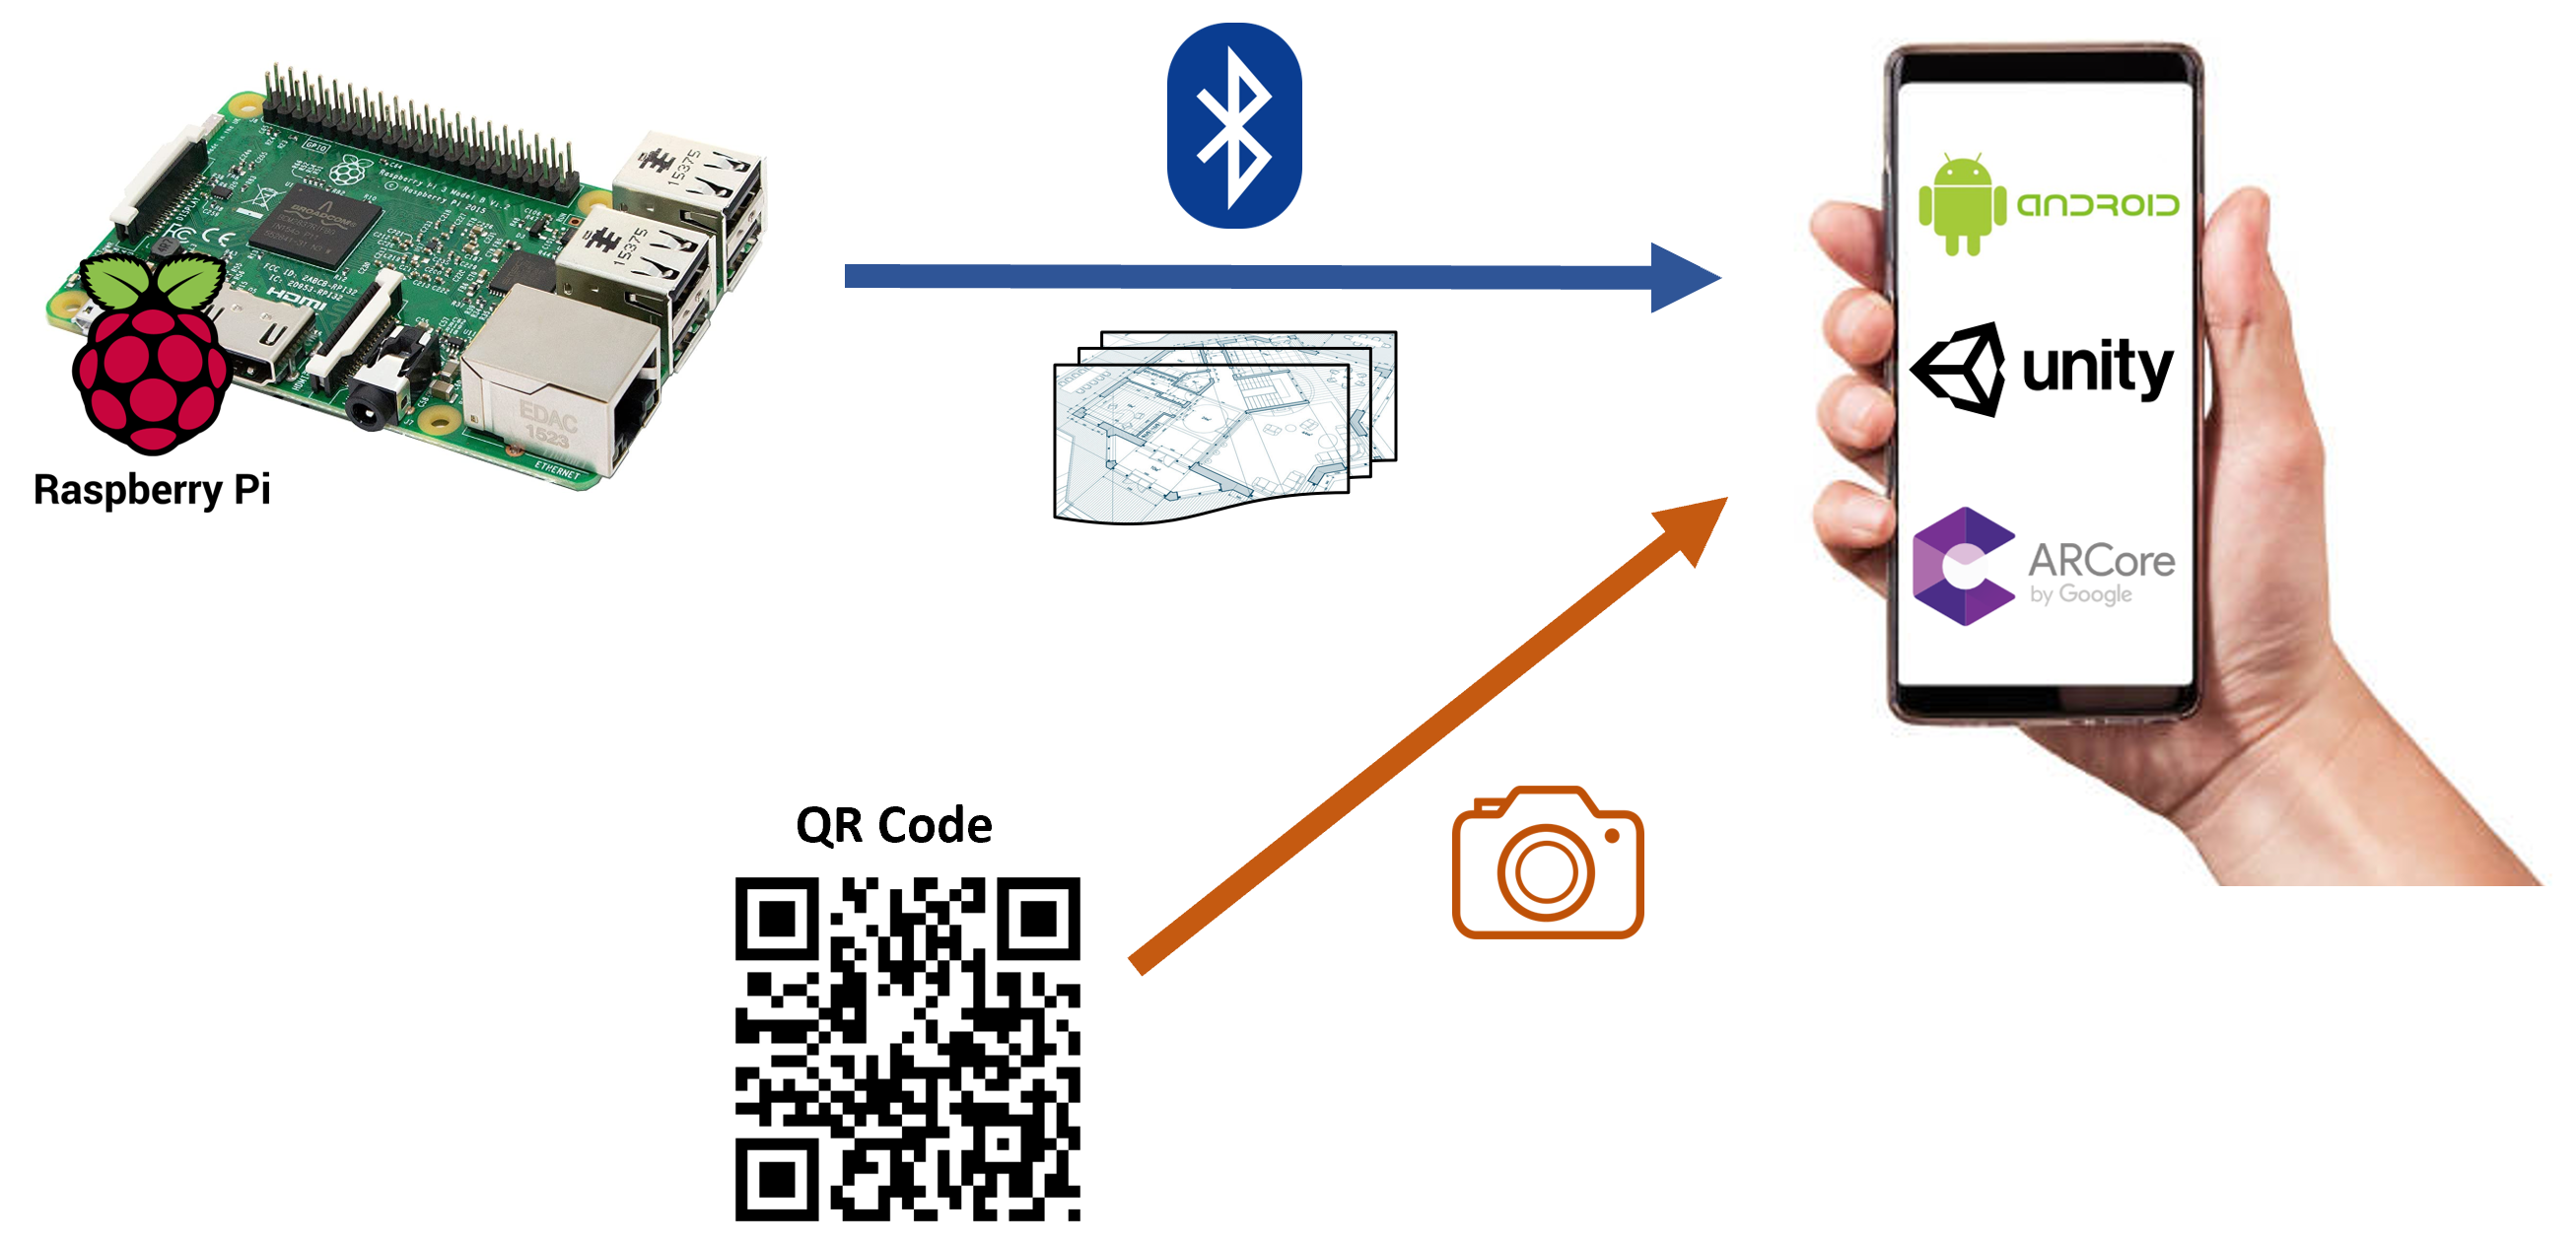
\includegraphics[width=\linewidth, keepaspectratio]{arquitectura_aplicacion}
    \caption{Arquitectura de la aplicación desarrollada.}
    \label{fig:arquitectura_aplicacion}
  \end{figure}

  %Por un lado, en ella se muestra la información de navegación, por otro, el usuario selecciona el destino deseado y configura la aplicación
  %el software utiliza los diversos sensores del teléfono, principalmente la cámara en combinación con sensores inerciales, para determinar la posición y orientación del teléfono a medida que éste se mueve en el espacio.
  %Como se detallará más adelante, el software utiliza los diversos sensores del teléfono, principalmente la cámara en combinación con sensores inerciales, para determinar la posición y orientación del teléfono a medida que éste se mueve en el espacio.

  \subsection{Software}

  El software de la aplicación se divide en dos, por un lado el del teléfono inteligente, por otro lado, el de la Raspberry Pi.

  Para el teléfono, se desarrolló una aplicación para Android en Unity.
  Unity es un motor de videojuego multiplataformas disponible como plataforma de desarrollo para Windows, Linux y Mac OS.
  Para este proyecto, se utilizó la versión de Unity 2019.4.22f1 en Windows 10.

  ARCore es una plataforma de Google para el desarrollo de aplicaciones de realidad aumentada.
  Hay tres funciones principales que ofrece ARCore: seguimiento de movimiento, comprensión del entorno (por ejemplo detección de superficies) y estimación de la iluminación.
  De estas tres funciones, para esta aplicación se utiliza la de seguimiento de movimiento.
  Ésta se basa en la identificación y seguimiento en el tiempo de puntos interesantes capturados por la cámara del teléfono en combinación con las lecturas de los sensores inerciales del teléfono como acelerómetros y giróscopos.
  El seguimiento de movimiento no sólo se utiliza para la navegación, sino también para poder colocar objetos, como flechas y pines, integrados en el mundo real de manera tal que, aunque el usuario se mueva y enfoque la cámara en otra dirección, el objeto virtual permanece fijo en su posición en el mundo real.
  Se utiliza para esta aplicación el kit de desarrollo de ARCore para Unity en su versión 1.23.0.

  Para la comunicación cliente-servidor con la Raspberry Pi, se utiliza el plugin de Unity \textit{Android \& Microcontrollers / Bluetooth} de TechTweaking que permite controlar fácilmente las capacidades Bluetooth del teléfono.

  \textit{Navmesh} es un conjunto de componentes que permiten la navegación en un ambiente tridimensional en Unity usando algoritmos de inteligencia artificial y en este proyecto se usa para encontrar el camino entre la ubicación actual y la ubicación deseada.

  El escaneo de los códigos QR para el reposicionamiento del usuario se logra con la librería ZXing para Unity.

  A la Raspberry Pi se le instala el sistema operativo Raspberry Pi OS basado en Debian.
  Para configurarla como servidor, se ejecuta un script de Python con el módulo \textit{PyBluez} que permite acceder a recursos Bluetooth de la máquina.
  La comunicación se realiza con protocolo RFCOMM (``Radio Frequency Communication") que permite emular la comunicación a través de puertos serie RS-232.
  Este protocolo es ampliamente utilizado por su simplicidad y porque permite adaptar aplicaciones que usan puertos serie fácilmente.

\end{standalone}
\end{document}
